\chapter{Theoretical Background}\label{Theoretical Background}
This first chapter wants to give an overview of all the theoretical concepts behind the methods that are applied in the second part of the thesis.
We are going to see what a time series is and what are the main statistical tools to analyze time series from a causal point of view.


% Sections:
% 1 Causal Inference for Time Series
% 2 State-of-the-art Methods
% 3 D2C, caD2C and TD2C
\section{Causality, Causal Inference \& Causal Discovery}
In this section we are going to define Causality and its derivations in mathematical and statistical fields.\\

We can define causality as the consequential relationship between two objects, a cause and an effect. A causal relationship underlines a connection, between two or more events, imposing a directionality, so that one of those events occurs, time-wise, before the others, and it can't be the other way around. J.Pearl - one of the greatest contributors in the causality field - proposed this simple definition: \textit{A causes B if B listens to A} (The Book of Why, Pearl \& Mackenzie, 2019). \\

Causality goes beyond the concept of correlation - \textit{correlation is not causation} - which only requires that two variables are connected and show dependency, but without imposing an order between them, i.e., one variable is not a consequence of the other, but just connected to it.\\
For the same reasons that discovering, analyzing and predicting the associations between variables is so important, knowing that we can (directly or indirectly) influence some aspects of the world we observe by controlling some of its features, is also quite attractive.
Aristotle, one of the most important philosophers of ancient Greece, believed that comprehending the causal structure of a process is a crucial element in understanding this process. (\cite{molak2023causal}). To cite another important philosopher, David Hume contended that causation relies on experience, which means any perceived cause-and-effect relationship could be erroneous. He maintained that since thoughts are subjective, it is impossible to definitively establish causality. Despite this quite skeptical interpretation of causality, we can still find, in statistical literature, some methods and techniques that aim to find strong enough evidences of consequential connections between events. From 1920 - when Sewall Wright, for the first time, put down mathematically the assumption that X causes Y and not the other way around (\ref{fig0}) (\cite{pearl2022causal}) - researchers started to develop an interest in what we today call Causal Learning. \\

\begin{figure}
    \centering
    \includegraphics[width=0.8\linewidth]{chapters/Images/Causality_vs_dependency.png}
    \caption{Dependency relation (a) and causality relation (b)}
    \label{fig0}
\end{figure}

Causal Learning encompasses two primary processes, both rely on observational or interventional data. The first, Causal Inference (Ci), aims to quantify the impact of a cause on its effect and relies heavily on a formal representation of the interactions among observed variables, called a causal graph. Despite its simplicity, this graphical representation is very effective for enhancing explainability. When the causal graph is unknown, it is possible to identify cause-effect pairs by integrating available data with prior knowledge. The second process, known as Causal Discovery (CD), aims to derive those causal connections within the system, it's a set of methods meant to recover the structure of the data-generating process from the data generated by that process. Recently, Causal Discovery has seen significant advancements, and this progress has led to the fragmentation of the field into various subfields, each with different assumptions, problems, and solutions, although they share the same ultimate goal (\cite{zanga2022survey}). Causal discovery methods and their application are at the core of this study and some of them are going to be deepened in section \ref{State-of-the-art Methods}.\\

\subsection{Simpson paradox and other examples and images to make causation more clear}
Here we display some examples to clarify the essential concept of causality, which may not be easily comprehended by someone who is used to thinking solely in terms of statistical correlation.
Let's start with one of the most famous effects of causation: the Simpson's paradox.
The paradox refers to the existence of data in which a statistical association that holds for an entire population is reversed in every subpopulation (i.e. considering subpupulations of data marked by a specifica variable's categories). This effect can help us a lot in understanding the logic behind causation because it shows us how a simple association between two variables can be denied and changed by considering a third variable that influences both the other two. 
Let's take, for example, three variables from a passed investigation about female smokers, their age, their smoker status (positive or negative) and their survival after 20 years from the first data collection (positive or negative). The marginal contingency table is here displayed:

\begin{table}[!ht]
    \centering
    \caption{Marginal table between the variables \textit{Smoker} and \textit{Survival state}. In green, the smallest survival rate between the two.}
    \begin{tabular}{r|ll}
        \textbf{} & \textbf{Alive} & \textbf{} \\ \hline
        \textbf{Smoker} & yes & no \\ \hline
        yes & 76,1\% & 23,9\% \\ 
        no & \color{Green}68,6\% & 31,4\% \\ 
    \end{tabular}
    \label{sp1}
\end{table}

As we notice in Table \ref{sp1}, smoking seems to favour the survival of considered subjects. In contrast, if we consider percentages in the partial contingency Table \ref{sp2} we see how this trend is reversed by including the third variable, \textit{Age}, and conditioning on it, i.e. by sorting data using its categories (1 = "Age $\leq 24$", 2 = "$24 <$ Age $\leq 65$", 3 = "Age $> 65$").

\begin{table}[!ht]
    \centering
    \caption{Partial contingency table, both in frequencies and percentages,  between the variables \textit{Smoker} and \textit{Survival state}, grouped by variable \textit{Age}. In green, the smallest survival rate per age category.}
    \begin{tabular}{r|ll|ll|ll}
        \multicolumn{7}{c}{\textbf{Percentages}} \\
        Age &  1 & ~ & 2 & ~ & 3 & ~ \\ \hline
        Smoker / Alive & yes & no & yes & no & yes & no \\ \hline
        yes & \color{Green}96.4\% & 3.6\% & \color{Green}80.3\% & 19.7\% & \color{Green}12.2\% & 87.8\% \\
        no & 98.6\% & 1.4\% & 84.5\% & 15.4\% & 13.9\% & 86.1\% \\
    \end{tabular}
    
    \vspace{1cm}
    
    \begin{tabular}{r|ll|ll|ll}
        \multicolumn{7}{c}{\textbf{Frequencies}} \\
        Age &  1 & ~ & 2 & ~ & 3 & ~ \\ \hline
        Smoker / Alive & yes & no & yes & no & yes & no \\ \hline
        yes & 53 & 2 & 384 & 94 & 6 & 43 \\
        no & 71 & 1 & 406 & 74 & 25 & 155 \\
    \end{tabular}
    \label{sp2}
\end{table}


Here, it's clear how smoking has a negative impact on survival rate in every age category. This is possible because, as we see also in \ref{fig6}, the variable \textit{Age} causes both the other two variables, and this changes their relation. This back-and-forth consideration of more variables can continue indefinitely, revealing a persistent challenge. Simple statistics cannot resolve this issue, as no statistical method alone can uncover the true causal relationships within the data. To determine the actual causal connections among the variables, we must first comprehend the underlying story and mechanisms that produced the observed results. Statisticians often interpret data with strong causal assumptions. In such cases, the paradox would disappear because the causal story could align with our example’s structure. However, even though the assumption that "smoking does not cause age" might seem obvious, it cannot be tested within the data itself. Moreover, causal information cannot be represented in contingency tables, which are frequently used for statistical inference. (\cite{pearl2016causal})\\

\textbf{\textit{Other examples}}\\

\subsection{Causality framework exploration}\label{Causality framework exploration}
Before proceeding, we would like to clarify, as completely as possible, all the statistical purposes bounded with the concept of causality. These purposes are in constant evolution, but we think it could be useful to portray the current state of this field to better understand the intents and the positioning in the literature of all the following topics.\\

As previously mentioned, causality learning objectives can be divided into two categories: determining causal effects, referred to as Causal Inference or Parameter Learning, and identifying causal relationships between objects, known as Causal Discovery or Structural Learning. Although these two areas intersect to some extent, their definitions differ slightly.
Understanding the causal relationships among variables typically involves determining the correct causal directions, causal lags, and associated causal indices. In contrast, learning about causal effects focuses on infer the impact of altering one variable on the outcome of another, given that some variables are already known to have causal connections.(\cite{chang2021multivariate})\\

These two purposes branch out, following various criteria, in different approaches. While studying causality and its application, the amount of methods in the literature could get confusing, that's why we provide, in Figure \ref{fig:1}, a concise summary of them in a schematic way.  

\begin{figure}[!h]
    \centering
    \includegraphics[width=1\linewidth]{chapters//Images/Causal Learning scheme.png}
    \caption{Ways of categorizing methods and approaches in Causal Learning context. In blue, we underlined TD2C's characteristic}
    \label{fig:1}
\end{figure}

\section{Fundamental tools}
This quite technical section is going to give us some important definitions that revolve around the Causality world. We dedicate this section of the thesis to theoretical concepts that require some specifications and that will be mentioned in the subsequent parts, or that are just useful to have a wider comprehension of the context.\\

We start with the definition of some fundamental concepts about causal relationships and causal effects.\\

\begin{definition}[Conditional Probability]
    Conditional Probability is the probability of one event, given that another event has occurred. $P(X|Y),$ where "$|$" stays for "given that".
\end{definition}
The complete notation is $P(X = x|Y = y)$: "the probability that the variable X takes the value x, given that the variable Y takes the value y". It can be also adapted to continuous cases, where we refer to probability densities.
\begin{definition}[Confounding]
    A confounding variable influences two or more other variables and produces a spurious association between them. From a purely statistical point of view, such associations are indistinguishable from the ones produced by a causal mechanism (\ref{fig6}).
\end{definition}

\begin{figure}[!h]
    \centering
    \includegraphics[width=0.7\linewidth]{chapters/Images/confounding.drawio.png}
    \caption{Example of confounding: from a first look (a) the increase in people going skiing at a certain time causes the decrease in sales of cucumbers, but, including the \textit{confounder} "winter season" (b), we are able to remove the causality between the previous two variables, since the new one causes them both.}
    \label{fig6}
\end{figure}

A very important aspect of a properly designed randomized experiment (RCT) is that it allows us to avoid confounding.
\begin{definition}[Intervention]\label{int}
     Intervention is changing one thing in the world and the observing whether and how this change affects another thing in the world.
\end{definition}

Interventions are the essence of scientific experiments. To describe interventions mathematically, we use the do-operator \ref{doo}: $P(Y = 1 | do(X = 0)$. While conditioning only modifies our view of the data, interventions affects the distribution by actively setting one (or more) variable(s) to a fixed value or distribution. \cite{molak2023causal}

\begin{definition}[Counterfactual]\label{count}
    Counterfactuals are estimates of how the world would look if we changed the value of one or more variables, holding everything else constant.
\end{definition}

Because, we can never observe the same event under two mutually exclusive conditions at the same time, counterfactuals cannot be observed, and so the true causal effect is always unknown. Two different counterfactual causal models can lead to the same interventional distribution.\\

Interventions and Counterfactuals, togheter with Associations, are the three steps of the so-called \textit{Ladder of Causation} described by Judea Pearl.
Each step answers to different causal questions:  association is related to observing, using association, we can answer questions about how seeing one thing changes our beliefs about another thing;  the action related to step two is doing (\ref{int}); activities associated with step three are imagining and understanding (\ref{count}).\\


\begin{definition}[do-operator]\label{doo}
    
\end{definition}

\textit{\textbf{Little digression on do-calcolus (Molak's book)}}\\

Then, we need some definitions about DAGs and SCMs.\\

\begin{definition}[Graph]
    A graph $G = (V, E)$ is a mathematical object represented by a tuple of two sets: a finite set of vertices $V$ and a finite set of edges $E \subseteq VV$. If not specified otherwise, this graph is intended as an undirected graph, where the undirected edge $(X, Y)$ is identical to the edge $(Y, X)$ and its graphical representation is $X - Y$.
\end{definition}

\begin{definition}[Directed Graph]
    A directed graph (DG) is a graph where the edge $(X, Y)$ is distinct from the edge $(Y, X)$.
\end{definition}
In particular, a directed edge $(X, Y)$ is graphically represented by an arrow as $X \rightarrow Y$, and induces a set of relationships between the vertices of the graph $G$. Given a vertex $X$, we denote by $Pa(X)$ its parents, i.e. the set of vertices that have an arrow into $X$, while we denote by $Ch(X)$ its children, i.e. the set of vertices that have an arrow out of $X$. Recursively, any parent and parent of a parent (child and child of a child) of $X$ is an ancestor $An(X)$ (descendant $De(X)$) of $X$.
The vertices connected to $X$ are said to be adjacent to $X$ and denoted by $Adj(X)$, while the vertices connected with an undirected edge are the neighbors $Ne(X)$. These two sets of vertices are identical in undirected graphs, but may be different in graphs with other mixed orientations.
\begin{definition}[Adjacency matrix]
    Adjacency matrices are square $M$ × $M$ matrices where $M$ is the number of nodes. Each positive entry in the matrix encodes an edge between a pair of nodes (\ref{fig7}).
\end{definition}

\begin{figure}[h!]
    \centering
    \begin{subfigure}[b]{0.45\textwidth}
        \centering
        \includegraphics[width=1.2\linewidth]{chapters/Images/DAG.png}
        \caption{}
        \label{fig:dag}
    \end{subfigure}
    \hfill
    \begin{subfigure}[b]{0.5\textwidth}
        \centering
        
        \[
        \renewcommand{\arraystretch}{2}
        \setlength{\arraycolsep}{1.5em}
        \begin{bmatrix}
        0 & \tcbox[colback=RubineRed, boxrule=0pt, arc=0pt, left=1pt, right=1pt, top=1pt, bottom=1pt]{1} & \tcbox[colback=NavyBlue, boxrule=0pt, arc=0pt, left=1pt, right=1pt, top=1pt, bottom=1pt]{1} & 0 \\
        0 & 0 & \tcbox[colback=Yellow, boxrule=0pt, arc=0pt, left=1pt, right=1pt, top=1pt, bottom=1pt]{1} & 0 \\
        0 & 0 & 0 & \tcbox[colback=Red, boxrule=0pt, arc=0pt, left=1pt, right=1pt, top=1pt, bottom=1pt]{1} \\
        0 & 0 & 0 & 0 \\
        \end{bmatrix}
        \]
        \caption{}
        \label{fig:adjacency-matrix}
    \end{subfigure}
    \caption{A Directed Acyclic Graph (a) and its Adjacency Matrix (b).}
    \label{fig7}
\end{figure}

\begin{definition}[Path (Directed path)]
    A path (Directed path) $\pi = (X - ... - Y)$ ($\pi = (X \rightarrow ... \rightarrow Y)$) is a tuple of non repeating vertices, where each vertex is connected to the next in the sequence with an undirected (directed) edge.
\end{definition}
\begin{definition} [Directd Acyclic Graph]: 
    A directed acyclic graph (DAG) is a directed graph G that has no cycles.
\end{definition}
\begin{definition}[Causal Graph]
    A causal graph $G = (V, E)$ is a graphical description of a system in terms of cause-effect relationships, i.e. the causal mechanism.
\end{definition}
\begin{definition}[Causal edge assumption]
    The value assigned to each $X$ is completely determined by the function $f$ given its parents: $X := f (Pa(X)) ∀X ∈ V$.
\end{definition}
\begin{definition}[Structural causal model]
    A structural causal model(SCM) is defined by the tuple $M = (V, U, F, P)$, where:
    \begin{itemize}
        \item $V$ is a set of endogenous variables, i.e. observable variables
        \item $U$ is a set of exogenous variables, i.e. unobservable variables, where $V \cap U = \emptyset$
        \item $F$ is a set of functions, where each function $f \in F$ is defined as $f_i : (V \cup U)^p \rightarrow V$, with $p$ the ariety of $f$, so that $f$ determines completely the value of $V_i$
        \item $P$ is a joint probability distribution over the exogenous variables $P(U) = \prod_i P(U_i)$.
    \end{itemize}
\end{definition}

SCMs consist of a set of exogenous (noise variables, root variables) and endogenous (observable variables) variables and a set of functions defining the relationships between these variables. They can be represented as graphs, with nodes representing variables and directed edges representing functions and they can produce interventional and counterfactual distributions. To represent a SCM we can use a set of equations or a graph, as in figure \ref{scm}.\\

\begin{figure}[!h]
\centering
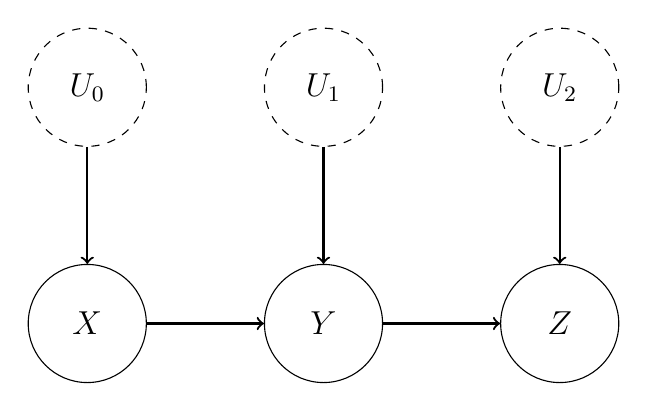
\begin{tikzpicture}[
  every node/.style={draw, circle, minimum size=1.5cm, font=\large},
  dashed node/.style={draw, circle, dashed, minimum size=1.5cm, font=\large},
  solid edge/.style={draw,->,thick}
]
% Define the nodes
\node[dashed node] (A) at (0,2) {$U_0$};
\node[dashed node] (B) at (3,2) {$U_1$};
\node[dashed node] (C) at (6,2) {$U_2$};
\node (D) at (0,-1) {$X$};
\node (E) at (3,-1) {$Y$};
\node (F) at (6,-1) {$Z$};
% Define the edges
\path[solid edge] (A) edge (D);
\path[solid edge] (B) edge (E);
\path[solid edge] (C) edge (F);
\path[solid edge] (D) edge (E);
\path[solid edge] (E) edge (F);
\end{tikzpicture}
\caption{An example of Structural Causal Model with exogenous (dashed circles) and endogenous (solid circles) variables}
\label{scm}
\end{figure}


\begin{definition}[Causal discovery problem]
    The causal discovery problem consists in recovering the groundtrouth graph $G^*$ (that generated $D$) from the given dataset $D$.
\end{definition}
\begin{definition}[Soundness and completeness of a Causal Discovery algorithm]
    A causal discovery algorithm is sound if it is able to solve the causal discovery problem, and it is complete if it outputs the most informative causal graph $G$ that can be recovered from the input dataset $D$, without making further assumptions.
\end{definition}
\begin{definition}[Markov property]\label{MP}
    A graph $G =(V, E)$ is said to satisfy the Markov property if the associated joint probability distribution $P(V)$ can be decomposed recursively as: $P(V) = \prod_{X \in V} P(X|Pa(X))$
\end{definition}
The probability factorization expressed in Definition \ref{MP} relies on the assumption that the relationships encoded by the graph match exactly the underlying conditional probability independencies:
$X \independent_P Y | Z \Rightarrow X \independent_G Y | Z$ where $Z$ is a subset of $V/{X, Y}$.
Essentially, it is assumed that the probability independence ($\independent_P$) implies the graphical independence ($\independent_G$).
\begin{definition}[Forks, Chains and Colliders]\label{fcc}
     Let $G =(V, E)$ be a DG and $\pi$ be a path on $G$. Then, given three vertices $X$, $Y$ and $Z$ in $\pi$, we have the following:
     \begin{itemize}
         \item $X\leftarrow Y \rightarrow Z$ is a fork on $\pi$
         \item $X \rightarrow Y \rightarrow Z$ is a chain on $\pi$
         \item $X \rightarrow Y \leftarrow Z$ is a collider on $\pi$
     \end{itemize}
\end{definition}

Testing for conditional independence (CI) between the variables is one of the most important techniques
to find the causal relationships among the variables (it is the core of \ref{Constraint-bsed Methods}). Conditional independence between two variables $X$ and
$Y$ results when they are independent of each other given a third variable $Z$ (i.e. $X \independent Y | Z$). In the case of causal discovery, CI testing allows deciding if any two variables are causally connected or disconnected. An important criterion for CI testing is the d-separation criterion which is formally defined in \ref{d-separation}.\\
Let's see an example: $X$ is conditionally independent of $Z$ given $Y$ i.e. $X \independent Z | Y$ in Figure \ref{3} (a) and in Figure \ref{3} (b), $X$ and $Z$ are independent, but are not conditionally independent given $Y$.\\ 

\begin{figure}[!h]
    \centering
    \includegraphics[width=1\linewidth]{chapters/Images/D-SEPARATION.png}
    \caption{Examples of fork and chain structures (a) and of d-separated DAG with a collider between $X$, $Y$ and $Z$ (b)}
    \label{3}
\end{figure}

\begin{definition}[d-separation]\label{d-separation}
    Let $G =(V, E)$ be a DG, $\pi$ be a path on $G$ and $Z$ a subset of $V$. The path $\pi$ is blocked by $Z$ if and only if $\pi$ contains:
    \begin{itemize}
        \item a fork $X \leftarrow Y \rightarrow Z$ or a chain $X \rightarrow Y \rightarrow Z$ such that the middle vertex $Y$ is in $Z$
        \item a collider $X \rightarrow Y \leftarrow Z$ such that middle vertex $Y$, or any descendant of it, is not in $Z$.
    \end{itemize}
\end{definition}

The set $Z$ d-separates $X$ from $Y$ if it blocks every path between $X$ and $Y$ (in \ref{3} (b) example, we have that $X$ and $W$ are d-separated considering the path that includes $Z$, but they become connected if we condition on this latter). When we say that a pair of nodes are d-separated, we mean that the variables they represent are definitely independent; when we say that a pair of nodes are d-connected, we mean that they are possibly, or most likely, dependent.\\

\textbf{\textit{see what to keep here below}}\\
In d-separation, the "d" stands for directional. This criterion offers a set of rules to determine if two variables are independent given a specific set of conditioning variables, which can be either a single variable or a collection of variables. Two variables with a directed edge ($\rightarrow$) between them are dependent. The set of testable implications provided by d-separation can be benchmarked with the available data $D$. If a graph $G$ might have been generated from a dataset $D$, then d-separation tells us which variables in $G$ must be independent conditional on other variables. If every d-separation condition matches a conditional independence in data, then no further test can refuse the model (\cite{pearl1988probabilistic}). If there is at least one path between two variables that is unblocked, then they are d-connected. If two variables are d-connected, then they are most likely dependent (except intransitive cases) (\cite{pearl1988probabilistic}). The d-separation or conditional independence between the variables in the key structures in \ref{fcc} follow some rules which are discussed below:\\
\begin{itemize}
    \item Conditional Independence in Chains: If there is only one unidirectional path between variables $X$ and $Z$, and $Y$ is any variable or set of variables that intercept that path, then $X$ and $Z$ are conditionally independent given $Y$ , i.e. $X \independent Z | Y$ .
    \item Conditional Independence in Forks: If a variable $X$ is a common cause of variables $Y$ and $Z$, and there is only one path between $Y$ and $Z$, then $Y$ and $Z$ are independent conditional on $X$, i.e. $Y \independent Z | X$.
    \item Conditional Independence in Colliders: If a variable $Z$ is the collision node between two variables $X$ and $Y$, and there is only one path between $X$ and $Y$ , then $X$ and $Y$ are unconditionally independent, i.e. $X \independent Y$. But, they become dependent when conditioned on $Z$ or any descendants of $Z$.
\end{itemize}

\begin{definition}[PDAG]
    The graph $G$ is a partially-directed acyclic graph (PDAG) if it can contain both undirected ($-$) and directed ($\rightarrow$) edges.
\end{definition}
\begin{definition}[Skeleton]
    Let $G$ be a PDAG. The skeleton of $G$ is the undirected graph resulting from changing any directed edge of $G$ to undirected.
\end{definition}
\begin{definition}[V-structure]
    Let $G$ be a PDAG. A v-structure in $G$ is a triple $X \rightarrow Y \leftarrow Z$ where $X$ and $Z$ are not adjacent. V-structures are also called unshielded colliders.
\end{definition}
\begin{definition}[Observational equivalence]
    Two DAGs $G$ and $H$ are observationally Markov equivalent if they have the same skeleton and the same V-structures, denoted as $G \equiv H$.
\end{definition}
\begin{definition}[Markov Equivalence Class]
    Two DAGs $G$ and $H$ belong to the same observational Markov equivalence class (MEC) if they are Markov equivalent. As generalization, the MEC of a graph $G$, denoted by $[G]$, represents the set of possible DAGs that are observationally equivalent.
\end{definition}
\begin{definition}[Markov Blanket]
    For any variable X, its Markov blanket (MB) is the set of variables such that X is independent of all other variables given MB. The members in the Markov blanket of any variable will include all of its parents, children, and spouses.
\end{definition}

Other useful definitions.

\begin{definition}[Lagged Causal Effect]
    Lagged Causal Effects refer to causal relationship between variables at the different time points.
\end{definition}
\begin{definition}[Instantaneous Causal Effect]
    Instantaneous Causal Effects refer to causal relationship between variables at the same time point.
\end{definition}
\begin{definition}[Expert knowledge]
    Expert knowledge is a term covering various types of knowledge that can help define or disambiguate causal relations between two or more variables.
\end{definition}
Depending on the context, expert knowledge might refer to knowledge from randomized controlled trials, laws of physics, a broad scope of experiences in a given area, and more.\\

We specify all the assumptions used by the methods in Section \ref{State-of-the-art Methods} to restrict their field of application.\\

\textbf{\textit{Molak e Pearl per approfondimenti e correzioni}}\\

\begin{definition}[Continuous-valued series]
    All series are assumed to have continuous-valued observations.
\end{definition}
However, many interesting data sources - such as social media posts or health states of an individual - are discrete-valued.
\begin{definition}[Causal Markov assumption]
    The causal Markov condition states that the node, V i , is independent of all its non-descendants (excluding its parents) given its parents. Therefore, formally, it can be presented as follows: $$V_i \independent_G \ V_j | PA(V_i) \ \  \forall \ \ j \neq i \in G(V, E) \symbol{92} \{ DE(V_i), PA(V_i) \}, $$ i.e., the node, $V_i$ , is independent of all other nodes in the graph, $G$ , excluding the descendants and parents of this node, given its parents. If this is not entirely clear to you at this stage, that’s perfectly fine.
\end{definition}
\begin{definition}[Linearity]
    The true data generating process, and correspondingly the causal effects of variables on each other, is assumed to be linear.
\end{definition}
 The value assigned to each variable $X_i$ is a linear function of the values already assigned to the earlier variables, plus a ‘disturbance’ (noise) term $e_i$, and plus an optional constant term $c_i$, that is $$X_i = \sum_{k(j)<k(i)} b_{ij}X_j + e_i + c_i$$
In reality, many real-world processes are nonlinear.
\begin{definition}[Discrete time] 
The sampling frequency is assumed to be on a discrete, regular grid matching the true causal time lag.
\end{definition}
If the data acquisition rate is slower or otherwise irregular, causal effects may not be identifiable. Likewise, the analysis of point processes or other continuous-time processes is precluded.
\begin{definition}[Known lag]
    The (linear) dependency on a history of lagged observations is assumed to have a known order. Classically, the order was not estimated and was taken to be uniform across all series.
\end{definition}
\begin{definition}[Stationariety]
    Some statistical properties of the time series do not change over time.
\end{definition}
\begin{definition}[Complete system]
    All relevant variables are assumed to be observed and included in the analysis - i.e., there are no unmeasured confounders.
\end{definition}
\begin{definition}[Absence of selection bias]
    
\end{definition}
\begin{definition}[Absence of feedback configurations]
\end{definition}
\begin{definition}[Sufficiency]
    All relevant variables are measured, and there are no hidden confounders.
\end{definition}
\begin{definition}[Perfectly observed]
     The variables need to be observed without measurement errors.
\end{definition}
\begin{definition}[Faithfulness]
    The observed independencies reflect the true causal structure, we write $$X \independent_P \ Y | Z \rightarrow X \independent_G \ Y | Z, $$ i.e., if $X$ and $Y$ are independent in the distribution given $Z$ , they will also be independent in the graph given $Z$.  
\end{definition}
It’s not very difficult to find situations where the assumption is violated. Intuitively, any situation where one variable influences another through two different paths and these paths cancel each other out completely would lead to the violation of faithfulness.
\begin{definition}[Non-Gaussianity]
    The noise terms are non-Gaussian.
\end{definition}
While the linear-Gaussian approach usually only leads to a set of possible models, equivalent in their conditional correlation structure, a linear-non-Gaussian setting allows the full causal model to be estimated, with no undetermined parameters.
\begin{definition}[No Instantaneous effects]
    Causes do not have immediate effects; there is a time lag between cause and effect.
\end{definition}
\begin{definition}[Time Homogeneity]
    The causal structure does not change over time.
\end{definition}
\begin{definition}[Additivity]
    The effect is a sum of the cause and an independent noise term.
\end{definition}
\begin{definition}[Sparsity]
    The causal graph is sparse, i.e., there are relatively few direct causal connections.
\end{definition}
\begin{definition}[No hidden confounders / Uncorrelated noise variables / Causal sufficience] 
    There are no unobserved variables that affect multiple observed variables; the unobserved noise variables are uncorrelated.
\end{definition}
\begin{definition}[Independence of noise terms]
    The noise terms in different causal mechanisms are independent, $$P(e_1, ..., e_n) = \prod_i P_i(e_i)$$
\end{definition}
\begin{definition}[Temporal order / Causal order]
    The cause precedes the effect in time. No later variable causes any earlier variable.
\end{definition}
\begin{definition}[Acyclicity]
    The causal graph has no cycles (it is a Directed Acyclic Graph, or DAG).
\end{definition}
\begin{definition}[Model Specification]
    The form of the causal relationships (e.g., linear, nonlinear) is correctly specified.
\end{definition}
\begin{definition}[Kernel assumption]
    The relationships can be captured in a high-dimensional feature space using kernel functions.
\end{definition}
\begin{definition}[Consistency]
    The method converges to the correct causal structure as the sample size increases.
\end{definition}
\begin{definition}[Causal minimality]
    The causal minimality assumption states that DAG G is minimal to distribution, P, if and only if G induces P, but no proper sub-graph of G induces P. In other words, if graph G induces P, removing any edge from G should result in a distribution that is different than P.
\end{definition}
Its implications have practical significance for constraint-based causal discovery methods (\ref{Constraint-bsed Methods}) and their ability to recover correct causal structures.
\begin{definition}[Identifiability]
    We say that a causal effect (or any other causal quantity) is identifiable when it can be computed unambiguously from a set of (passive) observations summarized by a distribution $P(V)$ and a causal graph $G$.
\end{definition}
In other words, if we have (1) enough information to control for non-causal information flow in the graph and (2) enough data to estimate the effect of interest, the effect is identifiable.
\begin{definition}[Positivity]
    Positivity assumptions comprehends two conditions: any estimator needs to have a large enough sample size to return meaningful estimates; the probability of every possible value of treatment in our dataset (possibly conditioned on all important covariates) is greater than 0.
\end{definition}
\begin{definition}[Exchangeability / Ignorability]
    The treated subjects, had they been untreated, would have experienced the same average outcome as the untreated did (being actually untreated) and vice versa. Formally: $$\{ Y^0, Y^1 \} \independent \ T|Z.$$ In the preceding formula, $Y^0$ and $Y^1$ are counterfactual outcomes under $T = 0$ and $T = 1$ respectively, and $Z$ is a vector of control variables.
\end{definition}

\textit{Examples from all possible sources}.\\


\section{Causal Inference for Time Series}
Before diving into the state-of-the-art section, it's important to underscore the difference between static and time-varying data (one of the possible cause of distinction in causality framework, as mentioned in \ref{Causality framework exploration}), from which derive two different types of approaches, with their different assumptions.\\

Let's start with the definition of Time Series Data.

\begin{definition}
Time Series data (TS) is a collection of observations measured over consistent
intervals of time. The observation of a Time Series variable $X_{j}$ at time t is denoted by $X^j_{t}$.
\end{definition}\\

Examples of time series data are retail sales, stock prices, climate data, heart rate of patients, brain activity recordings, temperature readings, daily delays of trains for a specific train station, number of ice-cream sold in a month by a supermarket, etc.\\

Discriminating between associative dependencies and effective causal relationships in high-dimensional and temporal settings, like time series data, presents significant challenges in causal inference from observational data. The multivariate interactions in these contexts generate substantial correlations among most variables.(\cite{bontempi2020learning}). 
Considering the potential confounding effects of additional variables is critical to truly discerning the causal relationships within such systems. For example, we can't assess, in a rigorous way, the causal influence of one variable $X_{i}$ on another $X_{j}$ without considering the influence of all other variables in the set $X \symbol{92} {Xi, Xj}$ , where $X$ is the set of all variables considered and the operator $\symbol{92}$ is the subtraction operator. This consideration is crucial because any of these variables, not included in the $(X_i,X_j)$ relationship, could confound it, possibly leading to incorrect conclusions. The unique challenges posed by time series data, due to potential latent confounding factors, are not fully addressed by bivariate models. This has necessitated the development of more sophisticated methods tailored to the complexities of time series analysis. The following section will illustrate some of these methods. (\cite{last paper on TD2C})\\

\textit{\textbf{Add something about it from intros in algos papers}}\\

\begin{figure}[!h]
\centering
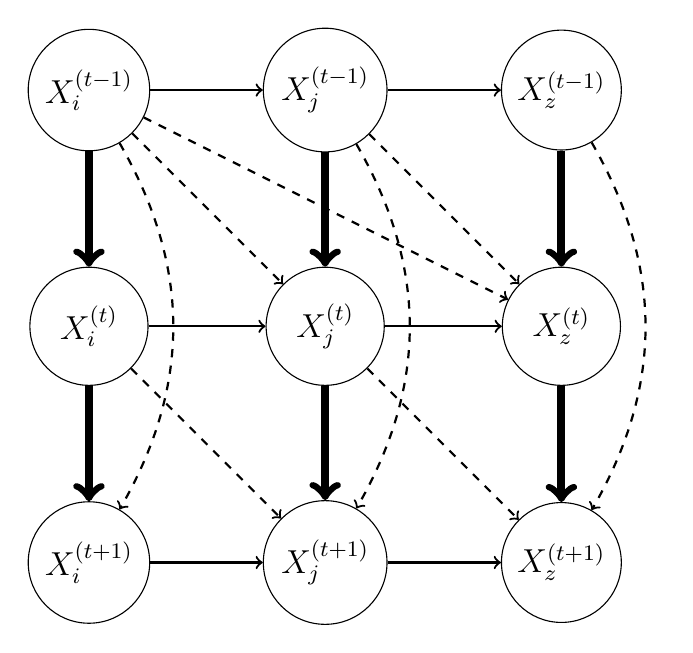
\begin{tikzpicture}[
  every node/.style={draw, circle, minimum size=1.5cm, font=\large},
  dashed edge/.style={draw,->,thick, dashed},
  solid edge/.style={draw,->,thick}
]
% Define the nodes
\node (A) at (0,2) {$X^{(t-1)}_i$};
\node (B) at (0,-1) {$X^{(t)}_i$};
\node (C) at (0,-4) {$X^{(t+1)}_i$};
\node (D) at (3,2) {$X^{(t-1)}_j$};
\node (E) at (3,-1) {$X^{(t)}_j$};
\node (F) at (3,-4) {$X^{(t+1)}_j$};
\node (G) at (6,2) {$X^{(t-1)}_z$};
\node (H) at (6,-1) {$X^{(t)}_z$};
\node (I) at (6,-4) {$X^{(t+1)}_z$};
% Define the edges
\path[solid edge, line width=1mm] (A) edge (B);
\path[solid edge, line width=1mm] (B) edge (C);
\path[solid edge, line width=1mm] (D) edge (E);
\path[solid edge, line width=1mm] (E) edge (F);
\path[solid edge, line width=1mm] (G) edge (H);
\path[solid edge, line width=1mm] (H) edge (I);
\path[solid edge] (A) edge (D);
\path[solid edge] (D) edge (G);
\path[solid edge] (B) edge (E);
\path[solid edge] (E) edge (H);
\path[solid edge] (C) edge (F);
\path[solid edge] (F) edge (I);
\path[dashed edge] (B) edge (F);
\path[dashed edge] (A) edge (H);
\path[dashed edge] (A) edge (E);
\path[dashed edge] (E) edge (I);
\path[dashed edge] (D) edge (H);
\path[dashed edge, bend left=30] (A) edge (C);
\path[dashed edge, bend left=30] (D) edge (F);
\path[dashed edge, bend left=30] (G) edge (I);
\end{tikzpicture}
\caption{An example of three time series variables, $X_i$, $X_j$, and $X_z$, connected through a fork structure. The thick solid lines represent the temporal effects of nodes on their immediate subsequent nodes. The thin solid lines represent the contemporaneous effects between nodes of different variables at the same instant. The dashed lines represent the lagged effects between nodes of different variables (or the same variable) at different (or the same) instants.}
\label{TS}
\end{figure}